%%%%%%%%%%%%%%%%%%%%%%%%%%%%%%%%%%%%%%%%%
% Uppsala University Assignment Title Page 
% LaTeX Template
% Version 1.0 (27/12/12)
%
% This template has been downloaded from:
% http://www.LaTeXTemplates.com
%
% Original author:
% WikiBooks (http://en.wikibooks.org/wiki/LaTeX/Title_Creation)
% Modified by Elsa Slattegard to fit Uppsala university
% License:
% CC BY-NC-SA 3.0 (http://creativecommons.org/licenses/by-nc-sa/3.0/)

%\title{Title page with logo}
%----------------------------------------------------------------------------------------
%	PACKAGES AND OTHER DOCUMENT CONFIGURATIONS
%----------------------------------------------------------------------------------------

\documentclass[12pt]{article}
\usepackage[english]{babel}
\usepackage[utf8x]{inputenc}
\usepackage{amsmath}
\usepackage{graphicx}
\usepackage{fontawesome}
\usepackage{float}
\setlength{\marginparwidth}{2cm}
\usepackage[colorinlistoftodos]{todonotes}
\usepackage[hidelinks]{hyperref}
\usepackage{subcaption}
\usepackage{multirow}
\usepackage{booktabs}
\usepackage{tabularx}
\usepackage{xcolor}
\usepackage{listings}

\definecolor{dkgreen}{rgb}{0,0.6,0}
\definecolor{gray2}{rgb}{0.5,0.5,0.5}
\definecolor{mauve}{rgb}{0.58,0,0.82}
\definecolor{backcolour}{rgb}{0.95,0.95,0.92}

\lstset{frame=tb,
  language=Python,
  aboveskip=3mm,
  belowskip=3mm,
  showstringspaces=false,
  columns=flexible,
  basicstyle={\small\ttfamily},
  numbers=left,
  numberstyle=\tiny\color{gray2},
  keywordstyle=\color{blue},
  commentstyle=\color{dkgreen},
  stringstyle=\color{mauve},
  backgroundcolor=\color{backcolour},
  breaklines=true,
  breakatwhitespace=true,
  tabsize=3,
  literate={å}{{\r a}}1 {ö}{{\"o}}1 {ä}{{\"a}}1 {Å}{{\r A}}1 {Ö}{{\"O}}1 {Ä}{{\"A}}1
}

\setlength\parindent{0pt}

\begin{document}

\begin{titlepage}

\newcommand{\HRule}{\rule{\linewidth}{0.5mm}} % Defines a new command for the horizontal lines, change thickness here

\center % Center everything on the page
 
%----------------------------------------------------------------------------------------
%	HEADING SECTIONS
%----------------------------------------------------------------------------------------

\begin{tikzpicture}[overlay, remember picture]
    \node[anchor=north west, xshift=1cm, yshift=-1cm] at (current page.north west)
    {
    
\includegraphics[width=2.5cm]{figs/titlepage/rexus_bexus_logo.jpg}
    
\includegraphics[width=2.5cm]{figs/titlepage/Uppsala_University_seal_svg.png}
    };
\end{tikzpicture}

\textsc{\LARGE REXUS/BEXUS}\\[1.5cm] % Name of your university/college

\includegraphics[scale=.2]{figs/titlepage/mirage_team_logo.png}\\[1cm] % Include a department/university logo - this will require the graphicx package
\textsc{\Large MIRAGE}\\[0.5cm] % Major heading such as course name
\textsc{\large Sensor Calibration}\\[0.5cm] % Minor heading such as course title

%----------------------------------------------------------------------------------------
%	TITLE SECTION
%----------------------------------------------------------------------------------------

\HRule \\[0.4cm]
{ \huge \bfseries Data Collection Instructions}\\[0.4cm] % Title of your document
\HRule \\[1.5cm]
 
%----------------------------------------------------------------------------------------
%	AUTHOR SECTION
%----------------------------------------------------------------------------------------

% \begin{minipage}{0.4\textwidth}
% \begin{flushleft} \large
% \emph{Author:}\\
% First name \textsc{Last name}\\ % Your name
% \end{flushleft}

% \end{minipage}\\[2cm]

% If you don't want a supervisor, uncomment the two lines below and remove the section above
\large \emph{Author:}\\
Olle \textsc{Hallberg}\\[1cm] % Your name

%----------------------------------------------------------------------------------------
%	DATE SECTION
%----------------------------------------------------------------------------------------

{\large \today}\\[2cm] % Date, change the \today to a set date if you want to be precise

\vfill % Fill the rest of the page with whitespace

\end{titlepage}

%----------------------------------------------------------------------------------------
%	SECTIONS SECTION
%----------------------------------------------------------------------------------------

\textit{This document serves as a navigation tool through the world of data collection. In this case, the data will be used by a calibration model to improve the measurements of the K96 NDIR gas sensor, used in the MIRAGE experiment.}

\tableofcontents
\newpage

\section{Introduction}
\subsection{Motivation}
The K96 output is affected by the concentration/molar fraction of methane, carbon dioxide and water, as expected. However, the K96 output is also influenced by environmental parameters such as temperature, humidity and pressure. The purpose of the calibration model is to mitigate the unwanted effects of the environmental parameters on the K96 output.\\

In order to train a calibration model in the form of a ML model, a training dataset is required. Furthermore, the training dataset must capture the effects of both the gas molar fraction and the environmental parameters on the K96 output.

\subsection{Previous Studies}\label{sec:previous_studies}
Multiple previous studies has been conducted on the calibration of the K96 using ML, in the following, three of them are be presented, focusing on the data collection.

\subsubsection*{\href{https://ieeexplore.ieee.org/abstract/document/11078940}{Accurate Measurements of Methane, Carbon Dioxide for Arctic and Wetland Conditions using NDIR Technology and AI-based Calibration \cite{11078940}}}

The \textbf{setup} used in the study is presented in Figure \ref{fig:accurate_measurments_setup}. A target gas (methane or carbon dioxide), dry air and humid air are mixed in a mixing chamber. The flow of each gas is controlled, enabling control of the molar fraction and humidity. A temperature coil enables control of the temperature. The mixed gas is ultimately measured by the K96 and a reference instrument.

\begin{figure}[htbp]
    \centering
    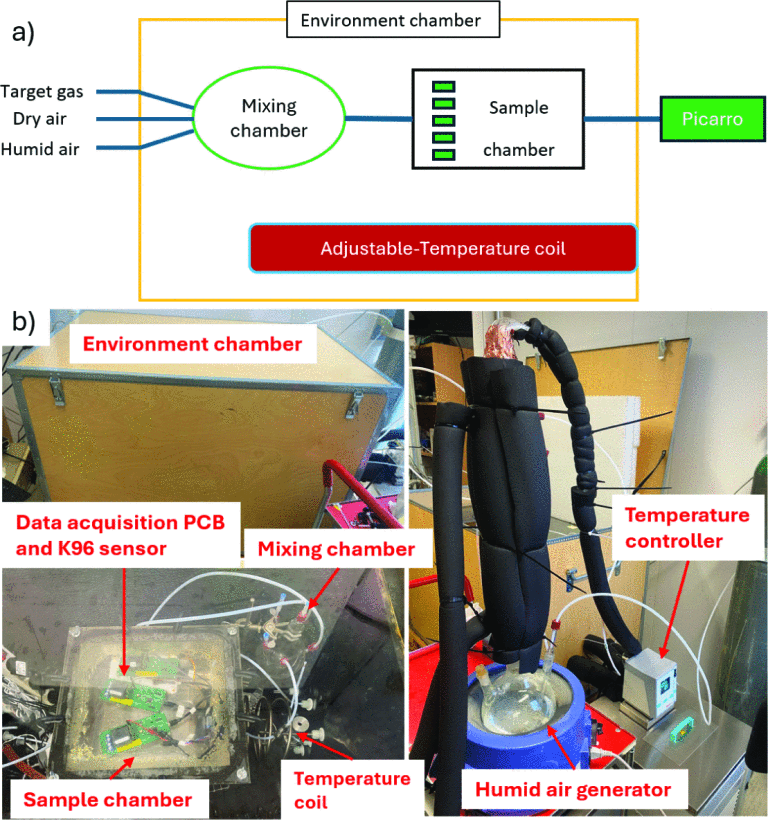
\includegraphics[width=1\linewidth]{figs/accurate_measurments/gia2-p6-gia-large.png}
    \caption{Setup used in reference \cite{11078940}. 
    % a) Theoretical setup. b) Practical setup.
    }
    \label{fig:accurate_measurments_setup}
\end{figure}

\begin{figure}[htbp]
\begin{subfigure}{0.49\textwidth}
    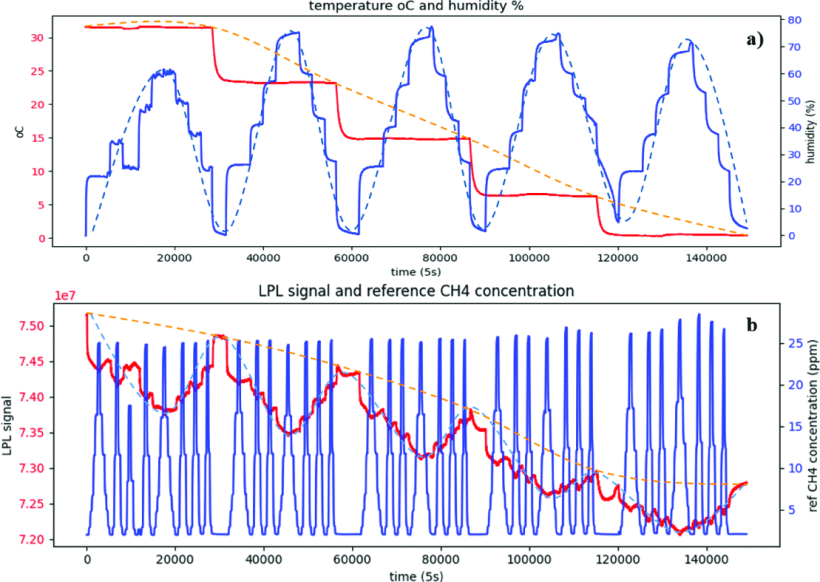
\includegraphics[width=0.9\linewidth]{figs/accurate_measurments/gia3-p6-gia-large.png} 
    \caption{For methane.}
    \label{fig:accurate_measurments_data_ch4}
\end{subfigure}
\begin{subfigure}{0.49\textwidth}
    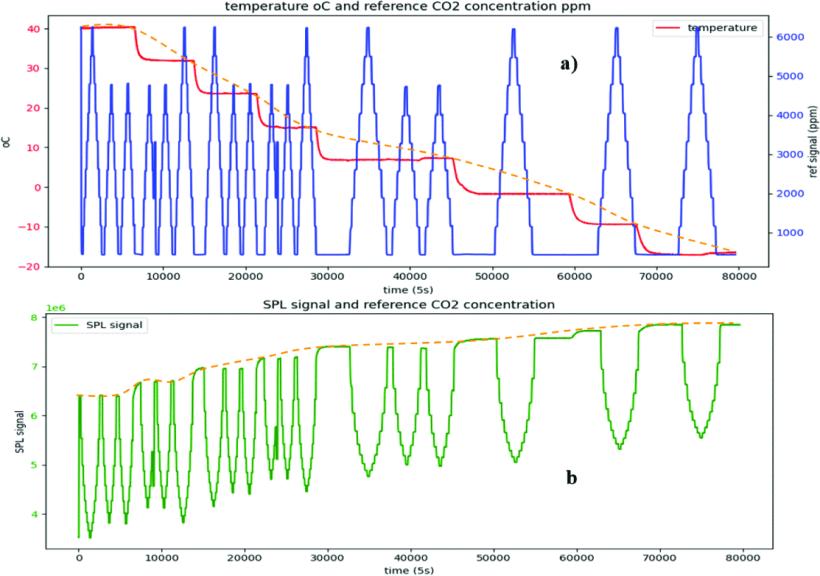
\includegraphics[width=0.9\linewidth]{figs/accurate_measurments/gia4-p6-gia-large.png}
    \caption{For carbon dioxide.}
    \label{fig:accurate_measurments_data_co2}
\end{subfigure}
\caption{Calibration datasets obtained in reference \cite{11078940}.}
\label{fig:accurate_measurments_data}
\end{figure}

The \textbf{calibration dataset}s obtained in the study are presented in Figure \ref{fig:accurate_measurments_data}. For methane, the temperature is varied with the lowest frequency, in steps. At each temperature step, the humidity is varied with a higher frequency, in steps. At each humidity step, the molar fraction is varied with the highest frequency. For carbon dioxide the procedure is the same, but without the variation of humidity.

\subsubsection*{\href{https://www.mdpi.com/1424-8220/25/24/7691}{Machine Learning-Enhanced NDIR Methane Sensing Solution for Robust Outdoor Continuous Monitoring Applications \cite{s25247691}}}

The \textbf{setup} used in the study is presented in Figure \ref{fig:ml_enhanced_setup}. One methane gas line and two nitrogen gas lines are used. One of the nitrogen gas lines is passed through a water bubbler to increase its humidity. The flow of each gas line is controlled, enabling control of the molar fraction and humidity. All gas lines enter a temperature-controlled oven, enabling control of the temperature. Inside the oven, the mixed gas is ultimately measured by the K96 and a reference instrument.

\begin{figure}[htbp]
    \centering
    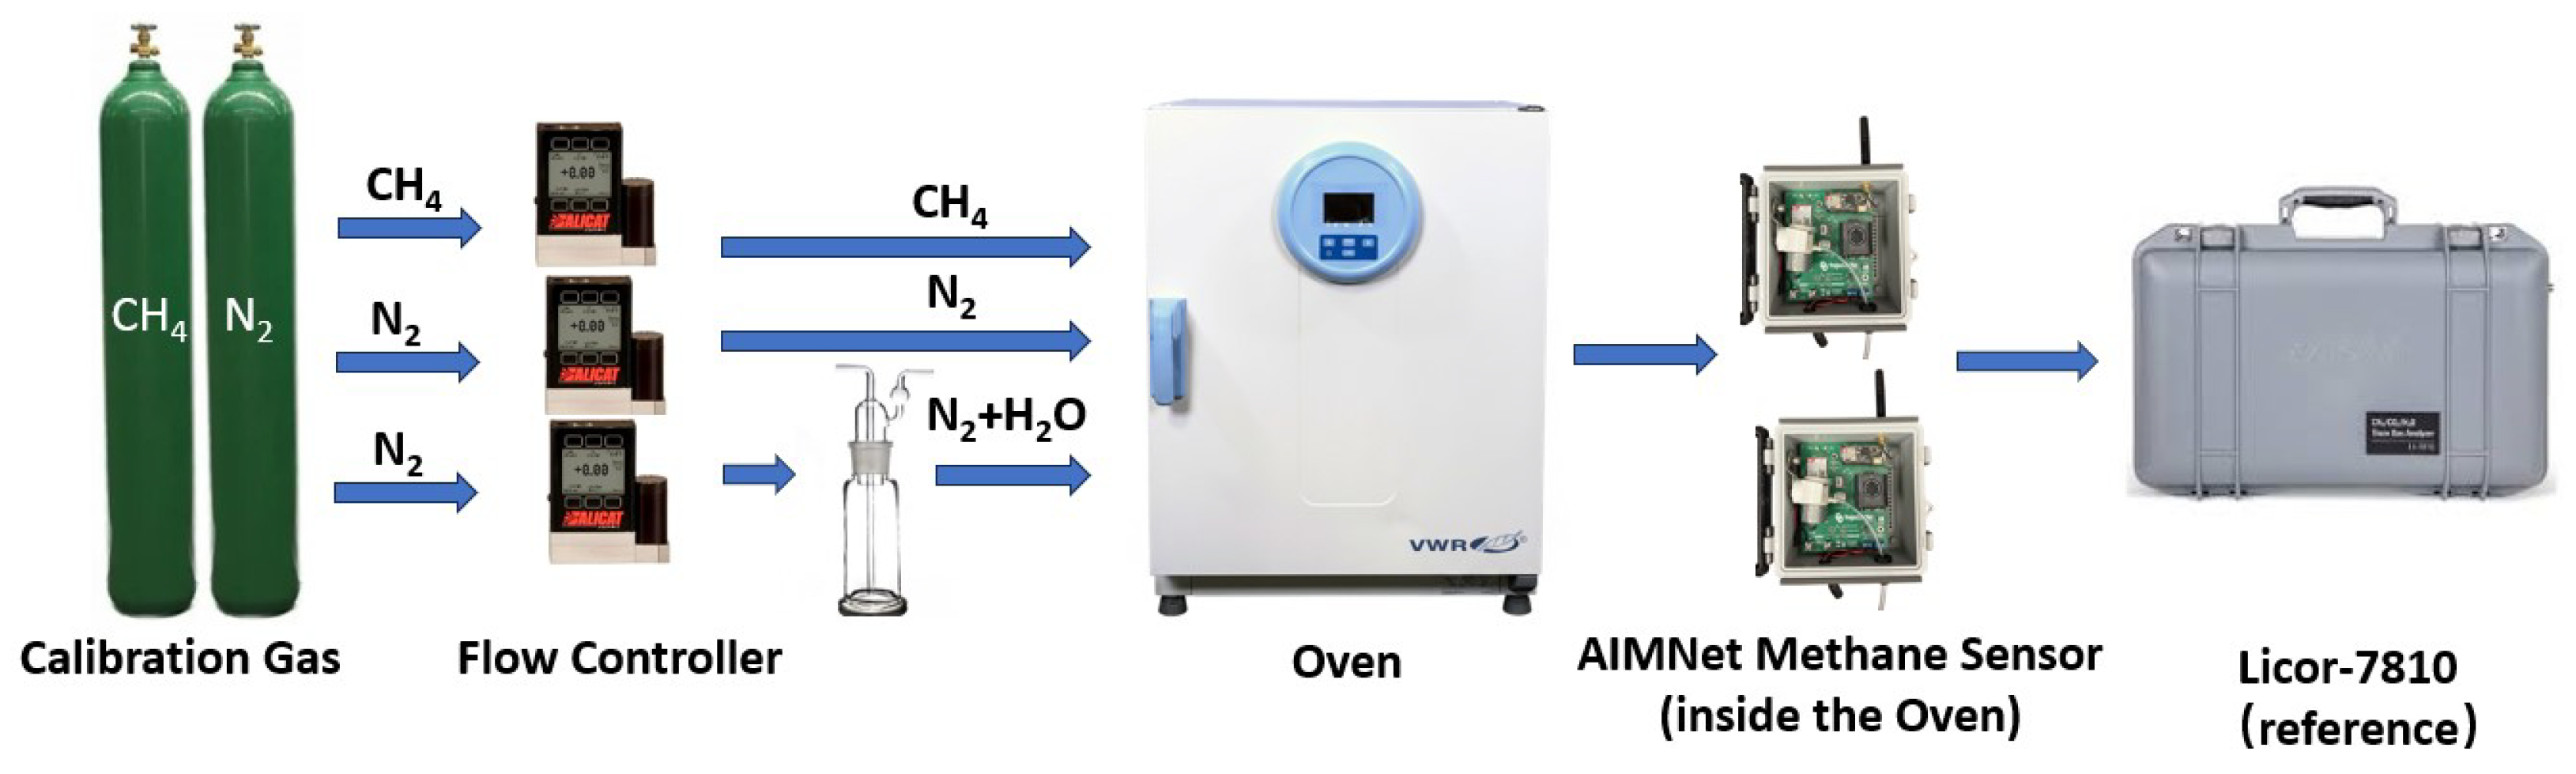
\includegraphics[width=1\linewidth]{figs/ml_enhanced/sensors-25-07691-g003.png}
    \caption{Setup used in reference \cite{s25247691}.}
    \label{fig:ml_enhanced_setup}
\end{figure}

\begin{figure}[htbp]
    \centering
    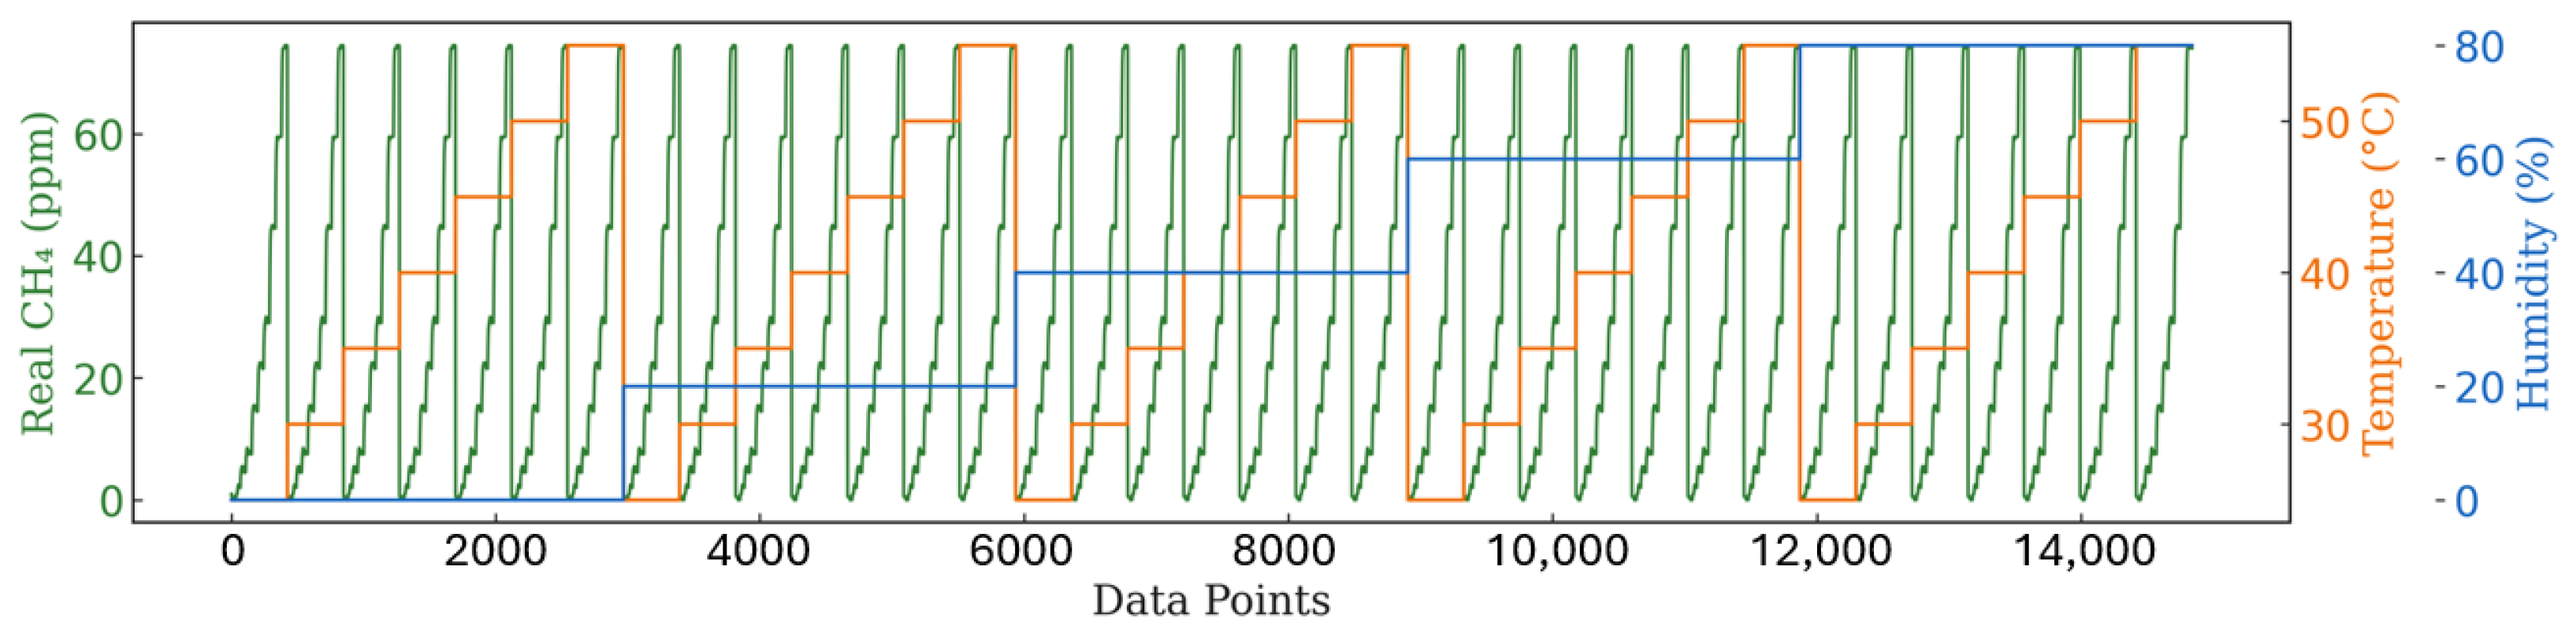
\includegraphics[width=1\linewidth]{figs/ml_enhanced/sensors-25-07691-g004.png}
    \caption{Calibration dataset obtained in reference \cite{s25247691}.}
    \label{fig:ml_enhanced_data}
\end{figure}

The \textbf{calibration dataset} obtained in the study is presented in Figure \ref{fig:ml_enhanced_data}. The humidity is varied with the lowest frequency, in steps. At each humidity step, the temperature is varied with a higher frequency, in steps. At each temperature step, the molar fraction is varied with the highest frequency, allowing several minutes at each step to ensure signal stabilization.

\subsubsection*{\href{http://urn.kb.se/resolve?urn=urn:nbn:se:uu:diva-592179}{Calibration of an NDIR Gas Sensor for Stratospheric Pressure and Temperature Conditions \cite{Olle2078608}}}

The \textbf{setup}s used in the study are presented in Figures \ref{fig:calibration_setup_dry_reference} and \ref{fig:calibration_setup_humid}. The setup for dry and reference instrument data uses a calibration gas (methane and carbon dioxide) and ambient air, respectively. A compressor pressurizes the gas into a pressure chamber covered with a heat blanket, enabling control of the pressure and temperature. Ultimately, the gas is measured by the K96, in the pressure chamber. The setup for humid data is the same, but with a dew point generator upstream of the compressor, enabling the control of the humidity.

\begin{figure}[htbp]
\begin{subfigure}{0.49\textwidth}
    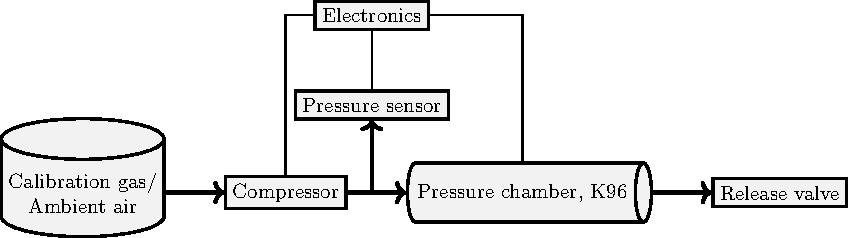
\includegraphics[width=0.9\linewidth]{figs/calibration/dry_reference_setup.pdf} 
    \caption{{\footnotesize For dry and reference instrument data}.}
    \label{fig:calibration_setup_dry_reference}
\end{subfigure}
\begin{subfigure}{0.49\textwidth}
    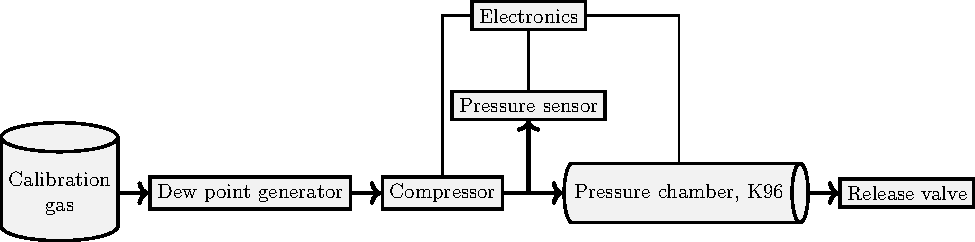
\includegraphics[width=0.9\linewidth]{figs/calibration/humid_setup.pdf} 
    \caption{For humid data.}
    \label{fig:calibration_setup_humid}
\end{subfigure}
\caption{Setups used in reference \cite{Olle2078608}.}
\label{fig:calibration_setup}
\end{figure}

\begin{figure}[htbp]
    \centering
    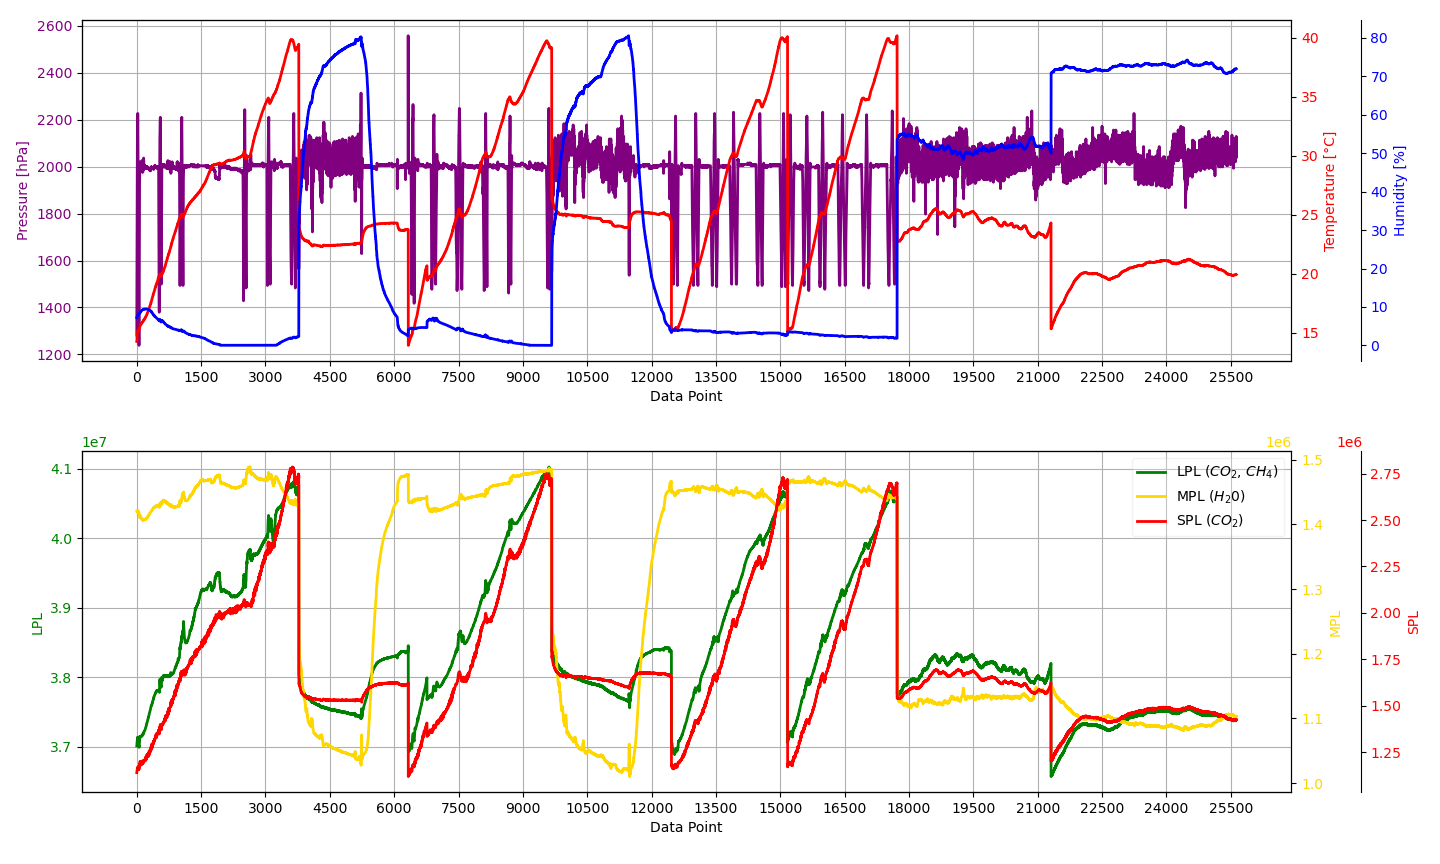
\includegraphics[width=1\linewidth]{figs/calibration/clean_data.png}
    \caption{Calibration dataset obtained in reference \cite{Olle2078608}.}
    \label{fig:calibration_data}
\end{figure}

The \textbf{calibration dataset} obtained in the study is presented in Figure \ref{fig:calibration_data}. For the dry data, were the humidity is somewhat constant and low, the molar fraction is varied with the lowest frequency, in steps. At each molar fraction step, the temperature is varied with a higher frequency, in steps. At each temperature step, the pressure is varied with the highest frequency. For the humid data, were the humidity reaches a peak and then decreases, the molar fraction is varied with the lowest frequency, in steps. At each molar fraction step, the humidity is varied, without the variation of temperature or pressure. For the reference instrument data, which is the last part of the dataset, no parameters are varied in steps.
\section{Method}
Analysing the previously conducted studies, presented in Section \ref{sec:previous_studies}, a couple of conclusions can be drawn. Regarding the setups, the incorporation of a reference instrument allows for a variation of molar fraction that does not demand calculations to find the true molar fraction. Regarding the calibration datasets, studies that vary the molar fraction with the highest frequency seem to obtain datasets with stronger correlation between the K96 output and the molar fraction as well as the environmental parameters.\\

With these conclusions in mind, the following presents, what seems to be, a desired calibration dataset and a setup which one hopefully can produce such a dataset with. Ultimately, a data analysis is presented to ensure the calibration dataset captures what is intended.

\subsection{Calibration dataset}
A general\footnote{In the sense that it captures the essence of the desired calibration dataset, without demanding the data collection to create an exact copy.} desired calibration dataset is presented in Figure \ref{fig:calibration_dataset}. The pressure is varied with the lowest frequency, in steps. At each pressure step, the temperature is varied with a higher frequency, in steps. At each temperature step, the molar fraction is varied with the highest frequency. 

\begin{figure}[htbp]
    \centering
    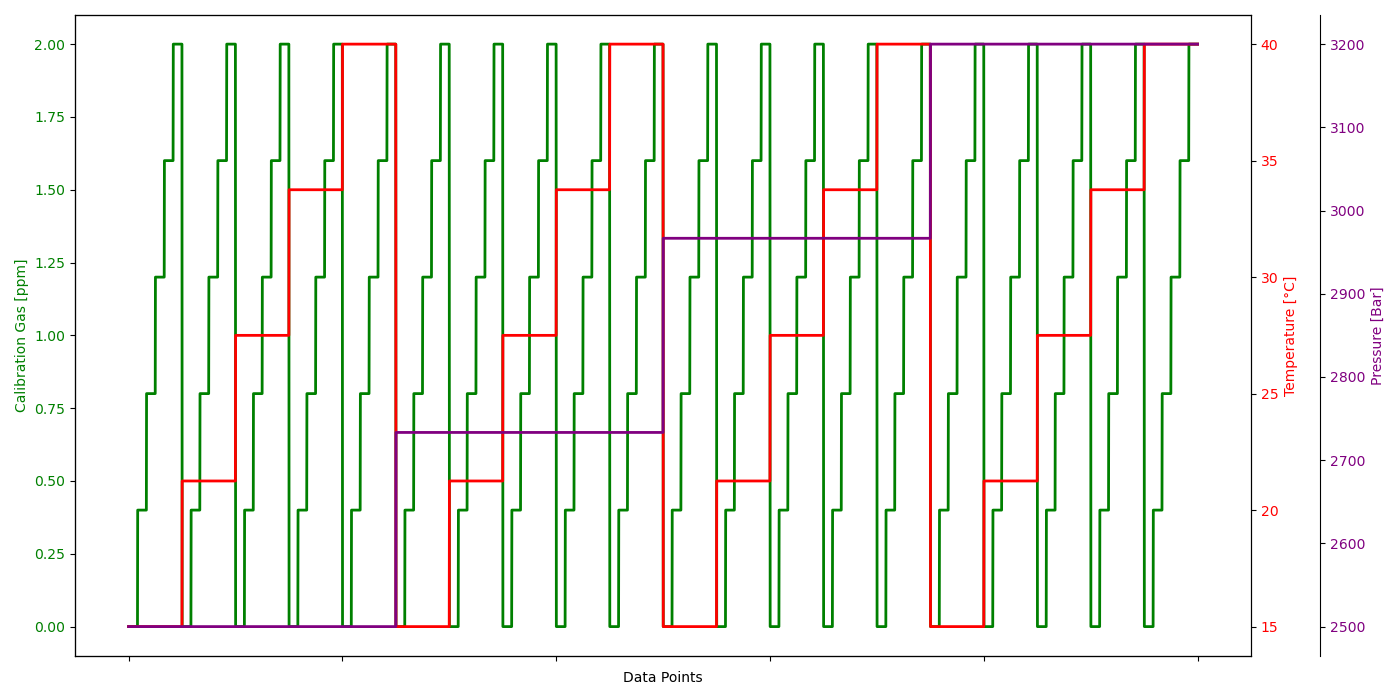
\includegraphics[width=1\linewidth]{figs/method/calibration_dataset.png}
    \caption{Calibration dataset.}
    \label{fig:calibration_dataset}
\end{figure}

The calibration dataset excludes a controlled variation of humidity. The reasoning behind this is that the inclusion of humidity will be hard to realise at the data collection facility\footnote{\href{https://www.icos-sweden.se/norunda}{ICOS SE Norunda research station}}. Also, a significant part of the MIRAGE flight will probably occur during low humidity conditions, due to the dry air at high altitudes.

\subsection{Setup}
A theoretical setup is presented in Figure \ref{fig:setup}.

\begin{figure}[htbp]
    \centering
    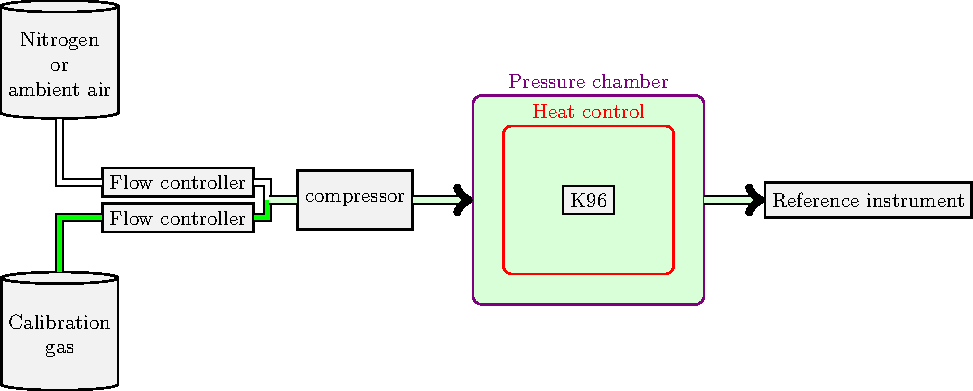
\includegraphics[width=1\linewidth]{figs/method/setup.pdf}
    \caption{Setup.}
    \label{fig:setup}
\end{figure}

Two gas lines are used. One for calibration gas containing methane and carbon dioxide and one for nitrogen gas or ambient air. The flow of each gas line is controlled before the lines are combined into one, enabling control of the molar fraction of the mixed gas. A compressor pressurizes the mixed gas into a pressure chamber, enabling control of the pressure. The pressure chamber possesses a heat control, enabling control of the temperature. The mixed gas is ultimately measured, by the K96 inside the pressure chamber, and by a reference instrument taking the mixed gas from the pressure chamber.

\subsection{Data Analysis}
During data collection, it is important to stop and analyse the data every so often, to ensure it captures what is intended. Therefore, the following presents requirements the calibration dataset must satisfy, and pseudocode that verify if the requirements are satisfied.

\subsubsection*{Requirements}
The requirements the calibration dataset must satisfy are presented in Table \ref{tab:requirements}.

\begin{table}[htbp]
    \centering
    \caption{Calibration dataset requirements.}
    \begin{tabularx}{\textwidth}{cX}
        \toprule
        Requirement & Description\\
        \midrule
        1 & The calibration dataset must capture the effect of the gas molar fraction on the K96 output.\\
        2 & The calibration dataset must capture the effect the environmental parameters on the K96 output.\\
        \bottomrule
    \end{tabularx}
    \label{tab:requirements}
\end{table}

The purpose of MIRAGE is to measure methane and carbon dioxide. Therefore requirement 1 ensures the calibration dataset captures the effects of the gases on the K96 output. The purpose of the calibration is to mitigate the unwanted effects of the environmental parameters on the K96 output. Therefore requirement 2 ensures the calibration dataset captures such unwanted effects.

\subsubsection*{Pseudocode}
The pseudocode that verify if the requirements are satisfied is presented in Listings \ref{lst:import}, \ref{lst:corr} and \ref{lst:scatter}.

\begin{lstlisting}[caption=Imports., label=lst:import]
import pandas as pd
import matplotlib.pyplot as plt

df = pd.read_csv("calibration_dataset.csv")
\end{lstlisting}

Listing \ref{lst:import} imports the required libraries and reads the calibration dataset, provided in a csv file.

\begin{lstlisting}[caption=Correlation matrix., label=lst:corr]
print(df[['gas_molar_fraction', 'environmental_parameters', 'k96_output']].corr())
\end{lstlisting}

Listing \ref{lst:corr} computes pairwise correlation between the gas molar fraction, the environmental parameters and the K96 output, and returns a correlation matrix.

\begin{lstlisting}[caption=Correlation scatter plots., label=lst:scatter]
fig, (ax1, ax2) = plt.subplots(1, 2)

ax1.scatter(df['gas_molar_fraction'], df['k96_output'], alpha=0.3)
ax1.set_xlabel('gas_molar_fraction [ppm]')
ax1.set_ylabel('k96_output')

ax2.scatter(df['environmental_parameters'], df['k96_output'], alpha=0.3)
ax2.set_xlabel('environmental_parameters')
ax2.set_ylabel('k96_output')

plt.tight_layout()
plt.show()
\end{lstlisting}

Listing \ref{lst:scatter} returns scatter plots of the gas molar fraction vs the K96 output and the environmental parameters vs the K96 output.
\vfill
\textit{This concludes the data collection instructions. For questions regarding this document, or \textbf{any} other matter, please do not hesitate to reach out.}\\

\begin{tabular}{l}
\href{mailto:olle.hallberg.3339@student.uu.se}{\raisebox{-0.05\height}\faEnvelope \ olle.hallberg.3339@student.uu.se}\\

\href{mailto:olle.hallberg02@gmail.com}{\raisebox{-0.05\height}\faEnvelope \ olle.hallberg02@gmail.com}\\

\href{tel:+46707809012}
{\raisebox{-0.05\height}\faPhone \ 
+46 70 780 90 12}
\end{tabular}

\newpage
\bibliographystyle{IEEEtran}
\bibliography{refs}

\end{document}